% χαρακτηριστικά κειμένου
\documentclass[11pt, a4paper]{article}
% Χρήση γλωσσών
\usepackage[utf8]{inputenc}
\usepackage[greek,english]{babel}
\usepackage{alphabeta}
\usepackage[LGR, T1]{fontenc}
\usepackage[parfill]{parskip}
\usepackage{amssymb}


\usepackage{amsmath}
% Χρήση Εικόνων
\usepackage{graphicx}
\graphicspath{ {./images/} }
%\usepackage{pgfplots}
% Εξώφυλλο
%\usepackage{graphicx}
\usepackage{subcaption}
\usepackage{mwe}
\usepackage{xcolor}
\usepackage{gensymb}
\usepackage{bm}
\usepackage[most]{tcolorbox}

\usepackage{minted}
\definecolor{bg}{rgb}{0.95,0.95,0.95}



%\usepackage[explicit]{titlesec}
%\usepackage{fourier}
%\usepackage{tikz}
%\usepackage{epigraph}
%\usepgflibrary{qrr.shapes.openrectangle}



%%% wglo turns glossaries on and off - for this purpose the package etoolbox is used
\usepackage{etoolbox}
\usepackage{framed}
\providetoggle{wglo}
\settoggle{wglo}{true}

\iftoggle{wglo}{%
 
    \usepackage[acronyms,nonumberlist]{glossaries-extra}
    \setabbreviationstyle[acronym]{long-short}
    \GlsXtrEnableEntryCounting{acronym}{0}
    
    \makeglossaries
    \newacronym{DSO}{DSO}{Distribution System Operator}
\newacronym{TSO}{TSO}{transmission system operator}
\newacronym{DER}{DER}{distributed energy resource}
\newacronym{PV}{PV}{photovoltaic}
\newacronym{EV}{EV}{electric vehicle}
\newacronym{WT}{WT}{wind turbine}
\newacronym{DG}{DG}{distributed generation}
\newacronym{LM}{LM}{Lagrange Multiplier}
\newacronym{DA}{DA}{day ahead}
\newacronym{DN}{DN}{distribution network}
\newacronym{TN}{TN}{transmission network}
\newacronym{DLMP}{DLMP}{distribution locational marginal price}
\newacronym{QP}{QP}{Quadratic Programming}
\newacronym{PoC}{PoC}{point of connection}
\newacronym{PI}{PI}{proportional-integral}
\newacronym{SoC}{SoC}{State of Charge}
\newacronym{PTDF}{PTDF}{power transfer distribution factor}
\newacronym{LNS}{LNS}{load not served}
\newacronym{RT}{RT}{Real-Time}
\newacronym{ToU}{ToU}{Time-of-Use}
\newacronym{MPC}{MPC}{Model Predictive Control}
}{%
    \newcommand{\gls}[1]{#1}
    \newcommand{\glspl}[1]{#1s}
}

\usepackage{nomencl}
\makenomenclature
%% This code creates the groups
% -----------------------------------------
\usepackage{etoolbox}
\renewcommand\nomgroup[1]{
  \item[\bfseries
  \ifstrequal{#1}{V}{Variables}{
  \ifstrequal{#1}{P}{Parameters}{
  \ifstrequal{#1}{A}{Indices and Sets}{}}}]}
% -----------------------------------------

% -----------------------------------------
\usepackage{libertine}

\title{\textbf{National Technical University of Athens} \\
School of Electrical \& Computer Engineering \\
\textbf{Programming Tools and Technologies for Data Science 2020-21} \\
Professors: \\ D. Fouskakis, N. Papaspyrou \\
\textbf{Exploratory Data Analysis using R}\\}
\author{Pantos Athanasios \\ Prospective MSc student \\ Α.Μ. ΕΔΕΜΜ: 03400026 \\
e-mail: pantos.thn@gmail.com}


\usepackage{listings}
\usepackage{color}

\definecolor{dkgreen}{rgb}{0,0.6,0}
\definecolor{gray}{rgb}{0.5,0.5,0.5}
\definecolor{mauve}{rgb}{0.58,0,0.82}

\lstset{frame=tb,
  language=R,
  backgroundcolor=\color{grey},
  aboveskip=3mm,
  belowskip=3mm,
  showstringspaces=false,
  columns=flexible,
  basicstyle={\small\ttfamily},
  numbers=none,
  numberstyle=\tiny\color{gray},
  keywordstyle=\color{blue},
  commentstyle=\color{dkgreen},
  stringstyle=\color{mauve},
  breaklines=true,
  breakatwhitespace=true,
  tabsize=3
}

%%%%%test

\usepackage{booktabs}
\usepackage{longtable}
\usepackage{array}
\usepackage{multirow}
\usepackage{wrapfig}
\usepackage{float}
\usepackage{colortbl}
\usepackage{pdflscape}
\usepackage{tabu}
\usepackage{threeparttable}
\usepackage{threeparttablex}
\usepackage[normalem]{ulem}
\usepackage{makecell}
\usepackage{xcolor}



\begin{document}

    \maketitle
    \thispagestyle{empty}
    \begin{center}
        
\includegraphics[width=8cm]{images/ntua.png}
    \end{center}
    \break
    \thispagestyle{empty}
    \tableofcontents
    
    \listoffigures
    
    \listoftables
    
    \clearpage
    \pagenumbering{arabic} 

%\begin{center}
    
%\end{center}
%\raggedright


\newpage
% στοίχιση δεξιά
%\raggedright



%\tableofcontents
%\input{nomenclature.tex}
\section{Introduction}

The coronavirus pandemic is undoubtedly the greatest challenge the world has faced in over a generation.

This is an analysis report of the Novel Coronavirus (COVID-19) around the world, to demonstrate data processing and visualisation with R, dplyr, data.table, tidyverse and ggplot2.

\subsection{Data Source}

The data source used for this analysis is the 2019 Novel Coronavirus COVID-19 (2019-nCoV) Data Repository
built by the Center for Systems Science and Engineering, Johns Hopkins University.

\subsection{R Packages}

Below is a list of R packages used for this analysis. Package magrittr is for pipe
and lubridate for date operations. Package tidyverse is a collection of R packages for data science, including
dplyr and tidyr for data processing and ggplot2 for graphics. Package gridExtra is for arranging multiple
grid-based plots on a page and kableExtra works together with kable() from knitr to build complex HTML
or LaTeX tables. Tidyquant is also used for its great aesthetics possibilities.

\begin{minted}[bgcolor=bg, fontsize=\scriptsize]{R}
library(magrittr) # pipe operations
library(lubridate) # date operations
library(tidyverse) # ggplot2, tidyr, dplyr...
library(gridExtra) # multiple grid-based plots on a page
library(ggforce) # accelerating ggplot2
library(kableExtra) # complex tables
library(data.table) # data analysis
library(tidyquant)  # for aesthetics
\end{minted}

\section{Loading Data}
At first, the data-sets, which are two CSV files, are downloaded and saved as local files and then are loaded into R. Fread function is used which is similar to data.table but faster and more convenient.

\begin{minted}[bgcolor=bg, fontsize=\scriptsize]{R}
#load the datasets
cases_df_raw <- fread("time_series_covid19_confirmed_global.csv", 
                   sep = ",", header= TRUE)
deaths_df_raw <- fread("time_series_covid19_deaths_global.csv", 
                   sep = ",", header= TRUE)
                   
dim(cases_df_raw)
dim(deaths_df_raw)
\end{minted}

## [1] 271 327 \newline
## [1] 271 327

Each data-set has 271 rows, corresponding to country/region/province/state. It has 150 columns. Starting
from column 5, each column corresponds to a single day. Here we have a look at the first 10 rows and the
first 10 columns.
\\
\\

\begin{table}[!h]

\caption{\label{tab:}Raw Data (Confirmed, First 10 Columns only)}
\centering
\fontsize{5}{7}\selectfont
\begin{tabular}[t]{llrrrrrrrr}
\toprule
Province/State & Country/Region & Lat & Long & 1/22/20 & 1/23/20 & 1/24/20 & 1/25/20 & 1/26/20 & 1/27/20\\
\midrule
\cellcolor{gray!6}{} & \cellcolor{gray!6}{Afghanistan} & \cellcolor{gray!6}{33.93911} & \cellcolor{gray!6}{67.70995} & \cellcolor{gray!6}{0} & \cellcolor{gray!6}{0} & \cellcolor{gray!6}{0} & \cellcolor{gray!6}{0} & \cellcolor{gray!6}{0} & \cellcolor{gray!6}{0}\\
 & Albania & 41.15330 & 20.16830 & 0 & 0 & 0 & 0 & 0 & 0\\
\cellcolor{gray!6}{} & \cellcolor{gray!6}{Algeria} & \cellcolor{gray!6}{28.03390} & \cellcolor{gray!6}{1.65960} & \cellcolor{gray!6}{0} & \cellcolor{gray!6}{0} & \cellcolor{gray!6}{0} & \cellcolor{gray!6}{0} & \cellcolor{gray!6}{0} & \cellcolor{gray!6}{0}\\
 & Andorra & 42.50630 & 1.52180 & 0 & 0 & 0 & 0 & 0 & 0\\
\cellcolor{gray!6}{} & \cellcolor{gray!6}{Angola} & \cellcolor{gray!6}{-11.20270} & \cellcolor{gray!6}{17.87390} & \cellcolor{gray!6}{0} & \cellcolor{gray!6}{0} & \cellcolor{gray!6}{0} & \cellcolor{gray!6}{0} & \cellcolor{gray!6}{0} & \cellcolor{gray!6}{0}\\
\addlinespace
 & Antigua and Barbuda & 17.06080 & -61.79640 & 0 & 0 & 0 & 0 & 0 & 0\\
\cellcolor{gray!6}{} & \cellcolor{gray!6}{Argentina} & \cellcolor{gray!6}{-38.41610} & \cellcolor{gray!6}{-63.61670} & \cellcolor{gray!6}{0} & \cellcolor{gray!6}{0} & \cellcolor{gray!6}{0} & \cellcolor{gray!6}{0} & \cellcolor{gray!6}{0} & \cellcolor{gray!6}{0}\\
 & Armenia & 40.06910 & 45.03820 & 0 & 0 & 0 & 0 & 0 & 0\\
\cellcolor{gray!6}{Australian Capital Territory} & \cellcolor{gray!6}{Australia} & \cellcolor{gray!6}{-35.47350} & \cellcolor{gray!6}{149.01240} & \cellcolor{gray!6}{0} & \cellcolor{gray!6}{0} & \cellcolor{gray!6}{0} & \cellcolor{gray!6}{0} & \cellcolor{gray!6}{0} & \cellcolor{gray!6}{0}\\
New South Wales & Australia & -33.86880 & 151.20930 & 0 & 0 & 0 & 0 & 3 & 4\\
\bottomrule
\end{tabular}
\end{table}

\begin{minted}[bgcolor=bg, fontsize=\scriptsize]{R}
#number of columns
n.col <- ncol(cases_df_raw)
#get dates from column names
dates <- names(cases_df_raw)[5:n.col] %>% substr(1,8) %>% mdy()

range(dates)
\end{minted}

[1] "2020-01-22" "2020-12-09"

It shows that the data was last downloaded on 09 Dec 2020 and all the stats and charts in this report are
based on that data.

\section{Data Preparation}
\subsection{Data Cleaning}

The two data sets are converted from wide to long format and then are aggregated by country. After that,
they are merged into one single data-set.Each step is well documented with comments in the code snippet below.


\begin{minted}[bgcolor=bg, fontsize=\scriptsize]{R}
# data cleaning and transformation
cleanData <- function(data) {
  #remove columns with names Province, State, Lat and Long and 
  #rename variable Country.Region to Country
  data <- data[ , -c("Province/State", "Lat", "Long")]
  data <- data %>% setnames(., old = "Country/Region",new = "Country")
  #convert from wide to long format
  data <- tidyr::gather(data, key=date, value=count, -Country)
  #convert the variable date from character to a date object
  data$date <- mdy(substr(data$date, 1, 8))
  #group by country and date
  data <- data.table(data)[, .(count = sum(count)), 
  by = list(date, Country)] %>%
  as.data.frame()
  return(data)
}

#apply the function to the two dataframes
data.confirmed <- cases_df_raw %>% cleanData() %>% 
  setnames(., old = "count", new = "confirmed")
data.deaths <- deaths_df_raw %>% cleanData() %>% 
  setnames(., old = "count", new = "deaths")

#merge the two datasets into one
data <- merge(data.confirmed, data.deaths, all=TRUE)

#sort by country and date
data <- setorder(data Country, date)

#daily increases of deaths and recovered cases
#set NA to the increases on day1
n <- nrow(data)
day1 <- min(data$date)

#create the daily confirmed cases and daily deaths
data <- data.table(data)[, .(date, Country, confirmed, deaths, 
                             confirmed.ind = ifelse(date == day1, 0,
                             confirmed - lag(confirmed, n=1)),
                             deaths.inc = ifelse(date == day1,0,
                                                 deaths - 
                                                 lag(deaths, n=1)))]
#change negative number of new cases to zero
data <- data.table(tt)[, .(date, Country, confirmed, deaths,
                   confirmed.ind  = ifelse(confirmed.ind  < 0, 0,
                                         confirmed.ind ),
                   deaths.inc = ifelse(deaths.inc < 0, 0, deaths.inc))
                   ]

#counts for the whole world
data.global <- data.table(data)[, .(
                     confirmed = sum(confirmed, na.rm=T),
                     deaths = sum(deaths, na.rm=T),
                     confirmed.ind = sum(confirmed.ind, na.rm=T),
                     deaths.inc = sum(deaths.inc,  na.rm=T)
                     ), by = list(date)]

#append to main daraframe
data <- rbind(data, data.global)
\end{minted}

We declare a function called cleanData. The only input argument is a data-set like the ones provided from John Hopkins University. This function is then applied to the two datasets provided by John Hopkins University. The following steps are done during the cleaning:

Below are the last 10 rows for Greece after the cleaning of the data set.

\begin{itemize}
	\item Columns with names Province, State, Lat and Long are removed.
	\item Variable Country.Region is renamed to Country.
	\item Data is converted from wide to long format.
	\item Variable date is converted from character to a date object via mdy function.
	\item Data is then grouped by country and date.
	\item Variable with the cumulative confirmed cases is named confirmed and
the variable with the cumulative number of deaths is named deaths.
	\item The two data-sets are then merged into one.
	\item Counts (confirmed and deaths) are calculated for the whole world.
	\item Two extra variables are created: confirmed.ind and deaths.inc with the
daily confirmed cases and daily deaths respectively.
\end{itemize}
\hspace{}
\newline
The last 10 rows based on Date column for Greece are displayed below after the cleaning has taken place.
\newline
\begin{table}[!h]
\caption{\label{tab:}Data after Cleaning for Greece}
\centering
\begin{tabular}[t]{lllrrrr}
\toprule
  & Country & date & confirmed & deaths & confirmed.ind & deaths.inc\\
\midrule
\cellcolor{gray!6}{314} & \cellcolor{gray!6}{Greece} & \cellcolor{gray!6}{2020-11-30} & \cellcolor{gray!6}{105,271} & \cellcolor{gray!6}{2,406} & \cellcolor{gray!6}{1,044} & \cellcolor{gray!6}{85}\\
315 & Greece & 2020-12-01 & 107,470 & 2,517 & 2,199 & 111\\
\cellcolor{gray!6}{316} & \cellcolor{gray!6}{Greece} & \cellcolor{gray!6}{2020-12-02} & \cellcolor{gray!6}{109,655} & \cellcolor{gray!6}{2,606} & \cellcolor{gray!6}{2,185} & \cellcolor{gray!6}{89}\\
317 & Greece & 2020-12-03 & 111,537 & 2,706 & 1,882 & 100\\
\cellcolor{gray!6}{318} & \cellcolor{gray!6}{Greece} & \cellcolor{gray!6}{2020-12-04} & \cellcolor{gray!6}{113,185} & \cellcolor{gray!6}{2,804} & \cellcolor{gray!6}{1,648} & \cellcolor{gray!6}{98}\\
\addlinespace
319 & Greece & 2020-12-05 & 114,568 & 2,902 & 1,383 & 98\\
\cellcolor{gray!6}{320} & \cellcolor{gray!6}{Greece} & \cellcolor{gray!6}{2020-12-06} & \cellcolor{gray!6}{115,471} & \cellcolor{gray!6}{3,003} & \cellcolor{gray!6}{903} & \cellcolor{gray!6}{101}\\
321 & Greece & 2020-12-07 & 116,721 & 3,092 & 1,250 & 89\\
\cellcolor{gray!6}{322} & \cellcolor{gray!6}{Greece} & \cellcolor{gray!6}{2020-12-08} & \cellcolor{gray!6}{118,045} & \cellcolor{gray!6}{3,194} & \cellcolor{gray!6}{1,324} & \cellcolor{gray!6}{102}\\
323 & Greece & 2020-12-09 & 119,720 & 3,289 & 1,675 & 95\\
\bottomrule
\end{tabular}
\end{table}


\clearpage
\subsection{Feature Engineering}

\begin{minted}[bgcolor=bg, fontsize=\scriptsize]{R}
#death rate
data %<>% mutate(death.rate = (100 * deaths / confirmed) %>% round(3))
#present confirmed cases
data %<>% mutate(present.confirmed = confirmed - deaths)
\end{minted}

The idea behind feature engineering is to first discover and then bring to the surface patterns in the data.
For this purpose two additional variables are calculated which could prove useful with our goal.
Specifically \colorbox{yellow!30}{death.rate} is the ration between the total dead and total confirmed cases while \colorbox{yellow!30}{present.confirmed} cases is calculated by simply subtracting confirmed cases from deaths.

\subsection{Variable Interpretation}

The data set contains daily information about covid-19 cases for every country in the world. Specifically it contains the cumulative confirmed cases (confirmed) as well as the deaths (deaths) for each country. The absolute number of confirmed (confirmed.ind) as well as deaths (deaths.inc) have been calculated, simply by subtracting  today's cumulative confirmed cases and deaths from those of the previous day.

Last but not least, death rate is simply the division of deaths by the number of confirmed cases while present confirmed is simply the subtraction of deaths from confirmed cases.

% Please add the following required packages to your document preamble:
% \usepackage{booktabs}
\begin{table}[!h]
\caption{\label{tab:}Data Table}
\centering
\begin{tabular}{@{}|l|l|l|@{}}
\toprule
Variable            & Variable Type & Value                                   \\ \midrule
date                & double        &                                         \\
Country             & character     & Greece, US, Germany etc.                \\
confirmed           & integer       &                                         \\
deaths              & integer       &                                         \\
confirmed.ind       & integer       &                                         \\
deaths.inc          & integer       &                                         \\
deaths.rate         & double        &                                         \\ 
present.confirmed   & integer       &                                         \\ \bottomrule
\end{tabular}
\end{table}

Confirmed cases are the number of people who have tested positive.

One of the stealthiest characteristics of the coronavirus is that it can be spread with little to no symptoms. This means that the number of people worldwide who are actually infected is probably much higher than the official confirmed cases.If you have not been tested, you are not counted.

Every country has its own methods for reporting, which include reviewing a patient's medical records and informing family members before releasing any figures.Leading infectious disease experts have already warned that, despite strict physical distancing measures, the world could still face hundreds of thousands of deaths - if not millions.
Just like confirmed cases, the actual number of deaths is almost certainly higher than what is being reported.

\section{Worldwide Cases}
After tidying up the data, we visualise it with various charts.

\subsection{Cumulative Number of Cases}

\begin{minted}[bgcolor=bg, fontsize=\scriptsize]{R}
#convert from wide to long format, for drawing area plots
data.long <- data %>%
  select(c(Country, date, confirmed, deaths)) %>%
  tidyr::gather(key=type, value=count, -c(Country, date))
global.long <- data.long %>% filter(Country == 'World')

data.global %<>% mutate(present.confirmed = confirmed - deaths,
                        death.rate = (100 * deaths / confirmed) 
                        %>% round(3))

#total cases and deaths
n_cases_worldwide <- global.long %>%
  ggplot(aes(x=date, y=count)) +
  geom_area(aes(fill=type), alpha=0.5) +
  labs(title=paste0('Numbers of Cases Worldwide')) +
  scale_fill_manual(values=c('green', 'red')) +
  theme_tq() + 
  scale_color_tq()

#log scale
n_cases_worldwide_log <- global.long %>%
  ggplot(aes(x=date, y=log(count))) +
  geom_area(aes(fill=type), alpha=0.5) +
  labs(title=paste0('Numbers of Cases Worldwide (log)')) +
  scale_fill_manual(values=c('green', 'red')) +
  theme_tq() + 
  scale_color_tq()
## show two plots side by side
grid.arrange(n_cases_worldwide, n_cases_worldwide_log, ncol=2)
\end{minted}
\newpage
\begin{figure}[h!]
    \centering
    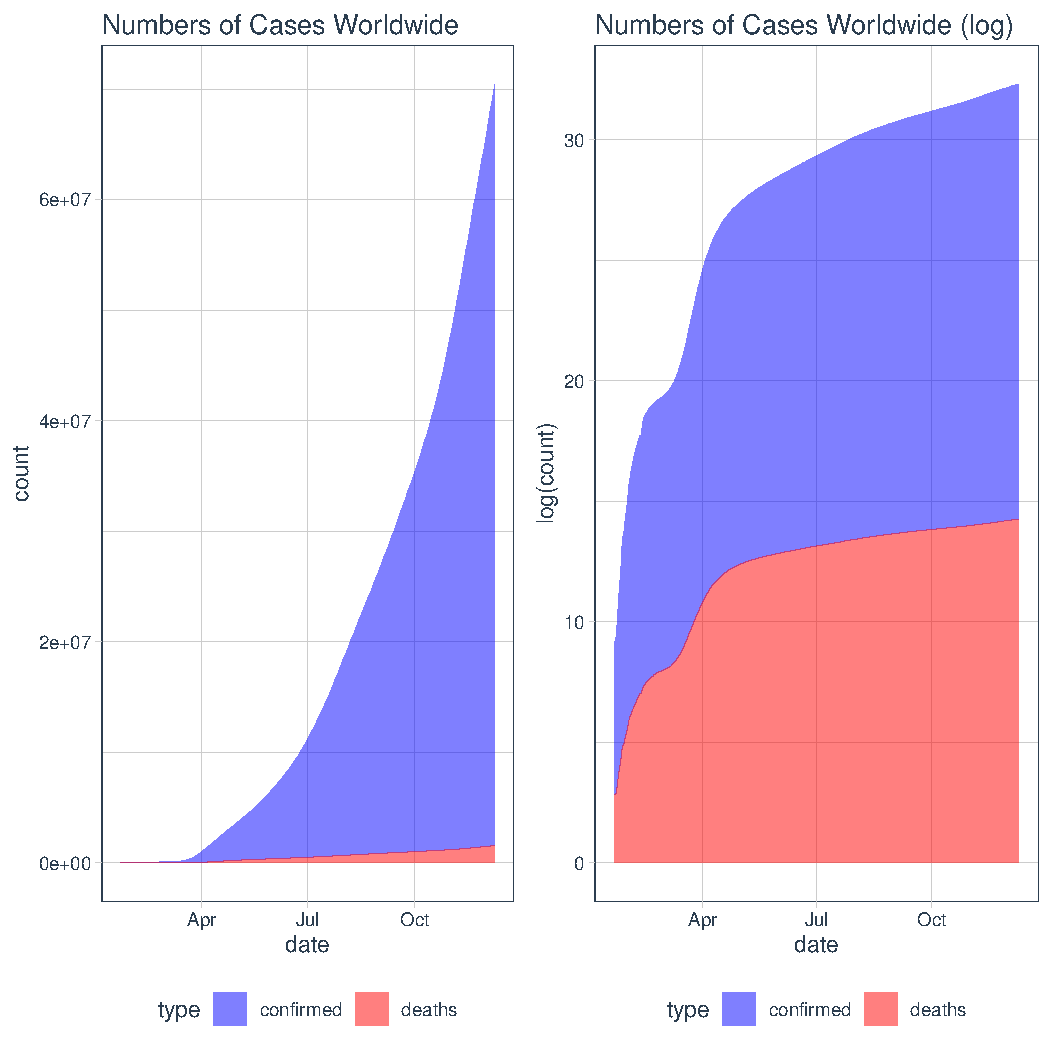
\includegraphics[width=\linewidth]{images/word_cases.pdf}
    \caption{World Cases}
    \label{fig:world_cases}
\end{figure}

As of 16:21 UTC on 22 December 2020, there are \colorbox{blue!30}{68,894,596} confirmed cases, and \colorbox{red!30}{1,569,374} deaths in 191 countries/territories

As you see in Figure \ref{fig:world_cases} the logarithmic scale is ideal for measuring rates of change, particularly rates of growth. On a logarithmic graph of COVID-19 infections, even though the overall numbers are still increasing, you can see the point at which the rate of growth starts to level off when that exponential growth has stopped.

In particular, it looks like that globally the rate of deaths has started to flatten and the number of cases is not growing as fast as it was during the first days of the pandemic. At that point, the logarithmic scale makes it possible to see when public health measures are starting to have the desired effect.

\newpage
\subsection{Daily Confirmed Cases \& Deaths}

\begin{minted}[bgcolor=bg, fontsize=\scriptsize]{R}
#world confirmed cases
current_confirmed_cases <- ggplot(data.global, 
                                  aes(x=date, y=present.confirmed)) +
  geom_point(shape=21) + geom_smooth(color = "blue", size =0.8) +
  geom_area(aes(fill=Country), show.legend = FALSE, alpha =0.3) +
  xlab('') + ylab('Count') + 
  labs(title='Current Confirmed Cases') +
  scale_fill_manual(values = 
                      c(rgb(0, 32, 150, maxColorValue = 255))) +
  theme(axis.text.x=element_text(angle=45, hjust=1)) +
  theme(legend.position = "none") +
  theme_tq() +
  scale_color_tq()

#daily new cases
daily_new_confirmed_cases <- ggplot(data.global, 
                                    aes(x=date, y=confirmed.ind)) +
  geom_point(size = 3, pch = 21, fill = "lightblue",
             color = "black") + 
  geom_smooth(size=1, span = 0.3, level = 0.99) +
  xlab('') + ylab('Count') + 
  labs(title='Daily New Confirmed Cases') +
  theme(axis.text.x=element_text(angle=45, hjust=1)) +
  scale_fill_manual(values = 
                      c(rgb(0, 32, 150, maxColorValue = 255))) +
  theme_tq() +
  scale_color_tq()
  
#world total deaths
current_deaths <- ggplot(data.global, aes(x=date, y=deaths)) +
  geom_point(shape=21) + geom_smooth(color="red", 
                                     size=0.8) +
  geom_area(aes(fill=Country), show.legend = FALSE, alpha =0.3) +
  xlab('') + ylab('Count') + 
  labs(title='Accumulative Deaths') +
  scale_fill_manual(values = 
                      c(rgb(255, 0, 0, maxColorValue = 255)), 
                    "#FF0000") +
  theme(axis.text.x=element_text(angle=45, hjust=1)) +
  theme_tq() +
  scale_color_tq()

#world daily deaths
current_daily_deaths <- ggplot(data.global, 
                               aes(x=date, y=deaths.inc)) +
  geom_point(size = 3, pch = 21, fill = "#FF9999",
             color = "black") + 
  geom_smooth(size=1, colour = 'red', span = 0.3,
              level = 0.99) +
  xlab('') + ylab('Count') + labs(title='Daily New Deaths') +
  theme(axis.text.x=element_text(angle=45, hjust=1)) +
  theme_tq() +
  scale_color_tq()

#display the 4 plots in a 2x2 matrix style
grid.arrange(current_confirmed_cases, daily_new_confirmed_cases,
             current_deaths, current_daily_deaths, ncol=2)
\end{minted}

\begin{figure}[h!]
    \centering
    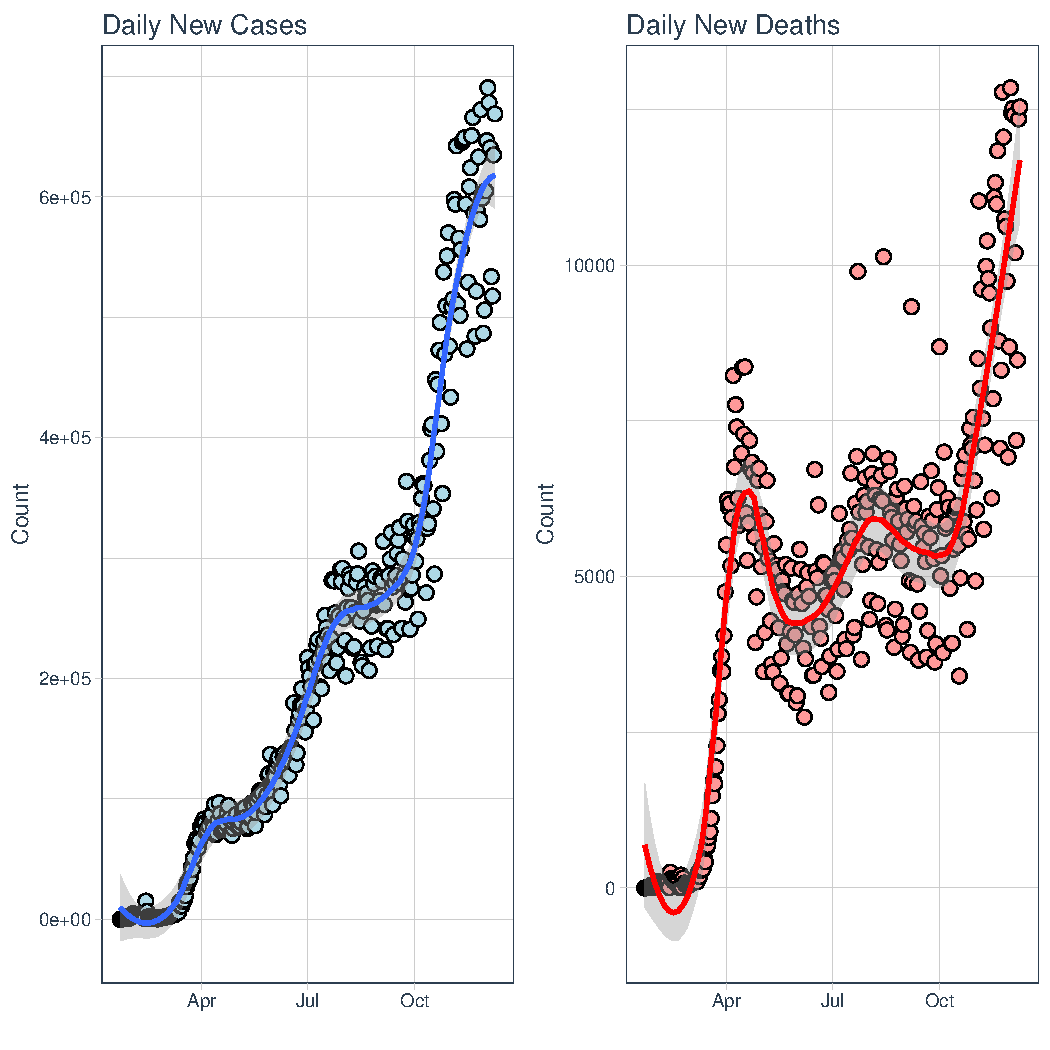
\includegraphics[width=\linewidth]{images/world_daily_confirmed_deaths_and_cases.pdf}
    \caption{Daily New Confirmed COVID-19 Cases /& Deaths}
    \label{fig:world_confirmed_cases}
\end{figure}

\textbf{Questions Figure \ref{fig:world_confirmed_cases}  answers:}

\textbf{Q. How widespread is the virus?}

\textbf{A.} Viruses, including COVID-19, tend to spread at an exponential rate, which means they multiply really quickly. On March 6, the world had 100,000 confirmed cases, one month later there were one million, and if the virus continues to grow at this rate, this number could reach 10 million by May.

\textbf{Q. Are the number of deaths increasing or decreasing?}

\textbf{A.} To answer this, you will need to look at the overall trends. If the slope is moving upwards, then deaths are increasing, if downwards then they are decreasing. Do not draw conclusions based on looking at daily changes on their own; these can differ based on how the data was collected the day before.

\newpage

\section{Top 20 Countries}

\subsection{Based on Confirmed cases}

\begin{minted}[bgcolor=bg, fontsize=\scriptsize]{R}
## ranking by confirmed cases world excluded
data.latest.all <- data %>% filter(date == max(date) & 
                                   Country != "World") %>%
  mutate(ranking = dense_rank(desc(confirmed)))

k <- 20
## top 20 countries: 21 excl. 'World'
top.countries <- data.latest.all %>% 
                filter(ranking <= k & Country != "World") %>%
                arrange(ranking) %>% pull(Country) %>% 
                as.character()

data.latest <- data.latest.all %>% 
               filter(!is.na(Country)) %>%
               mutate(Country=ifelse(ranking <= k,
                      as.character(Country), 'Others')) %>%
               mutate(Country=Country %>% 
               factor(levels=c(top.countries, 'Others')))

data.latest %<>% group_by(Country) %>%
  summarise(confirmed=sum(confirmed), confirmed.ind=sum(confirmed.ind),
            present.confirmed=sum(present.confirmed), 
            deaths=sum(deaths), deaths.inc=sum(deaths.inc)) %>%
  mutate(death.rate=(100 * deaths/confirmed) %>% round(1))

data.latest %<>% select(c(Country, confirmed, deaths, death.rate,
                 confirmed.ind, deaths.inc, present.confirmed))

data.latest %>% mutate(death.rate=death.rate %>% 
                format(nsmall=1) %>% paste0('%')) %>%
  kable('latex', booktabs=T, row.names=T, align=c('l', rep('r', 6)),
        caption=paste0('Cases in Top 20 Countries - ', max.date,
                       '.'),
        format.args=list(big.mark=',')) %>%
  kable_styling(font_size=7, latex_options=c('striped', 
                                             'hold_position', 
                                             'repeat_header'))
\end{minted}

\newpage
\begin{figure}[h!]
    \centering
    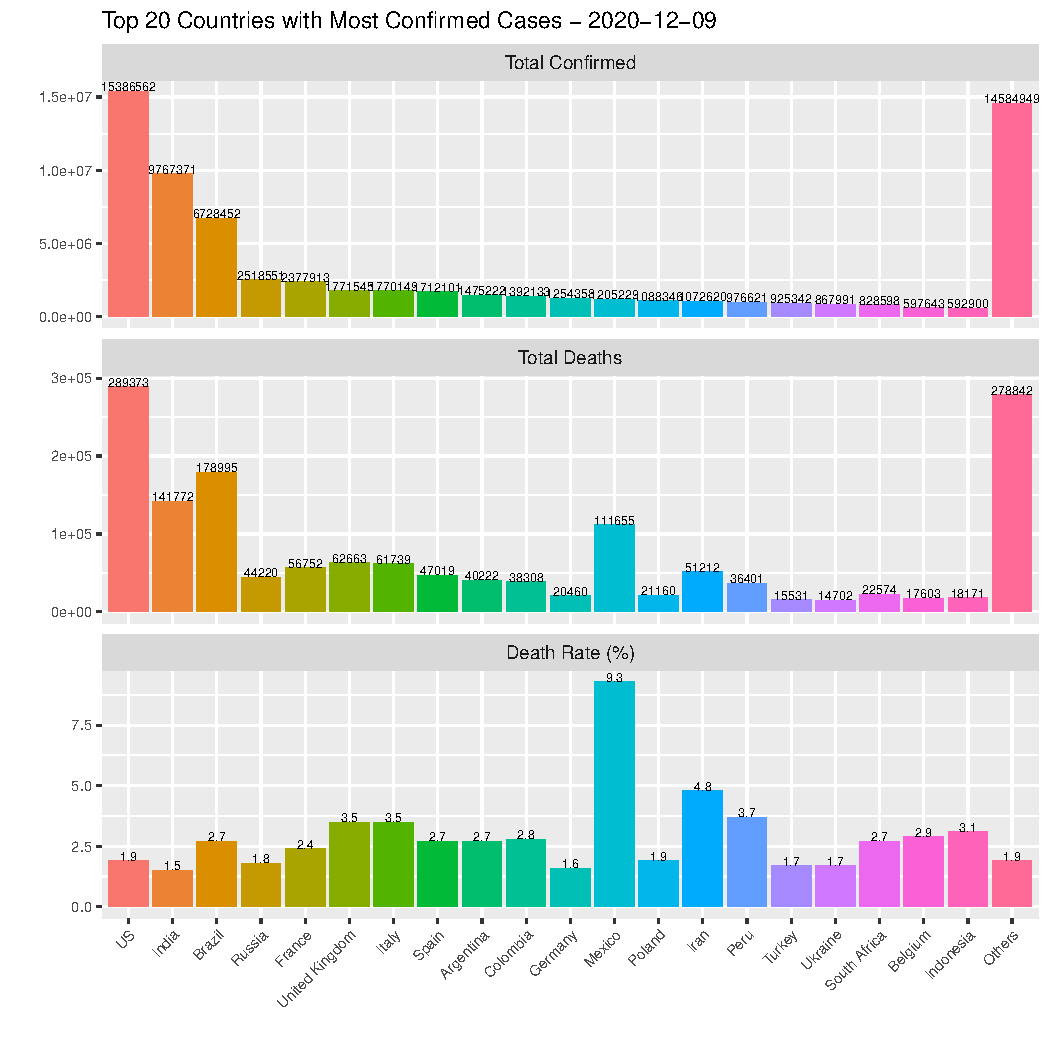
\includegraphics[width=\linewidth]{images/bar_chart.pdf}
    \caption{Bar Chart}
    \label{fig:bar_chart}
\end{figure}

\begin{table}[!h]
\caption{\label{tab:} Number of Cases in Top 20 Countries - 2020-12-09.}
\centering
\fontsize{7}{9}\selectfont
\begin{tabular}[t]{llrrrrrr}
\toprule
  & Country & confirmed & deaths & death.rate & confirmed.ind & deaths.inc & present.confirmed\\
\midrule
\cellcolor{gray!6}{1} & \cellcolor{gray!6}{US} & \cellcolor{gray!6}{15,386,562} & \cellcolor{gray!6}{289,373} & \cellcolor{gray!6}{1.9\%} & \cellcolor{gray!6}{221,267} & \cellcolor{gray!6}{3,124} & \cellcolor{gray!6}{15,097,189}\\
2 & India & 9,767,371 & 141,772 & 1.5\% & 31,521 & 412 & 9,625,599\\
\cellcolor{gray!6}{3} & \cellcolor{gray!6}{Brazil} & \cellcolor{gray!6}{6,728,452} & \cellcolor{gray!6}{178,995} & \cellcolor{gray!6}{2.7\%} & \cellcolor{gray!6}{53,453} & \cellcolor{gray!6}{836} & \cellcolor{gray!6}{6,549,457}\\
4 & Russia & 2,518,551 & 44,220 & 1.8\% & 25,838 & 546 & 2,474,331\\
\cellcolor{gray!6}{5} & \cellcolor{gray!6}{France} & \cellcolor{gray!6}{2,377,913} & \cellcolor{gray!6}{56,752} & \cellcolor{gray!6}{2.4\%} & \cellcolor{gray!6}{14,717} & \cellcolor{gray!6}{299} & \cellcolor{gray!6}{2,321,161}\\
\addlinespace
6 & United Kingdom & 1,771,545 & 62,663 & 3.5\% & 16,634 & 533 & 1,708,882\\
\cellcolor{gray!6}{7} & \cellcolor{gray!6}{Italy} & \cellcolor{gray!6}{1,770,149} & \cellcolor{gray!6}{61,739} & \cellcolor{gray!6}{3.5\%} & \cellcolor{gray!6}{12,755} & \cellcolor{gray!6}{499} & \cellcolor{gray!6}{1,708,410}\\
8 & Spain & 1,712,101 & 47,019 & 2.7\% & 9,773 & 373 & 1,665,082\\
\cellcolor{gray!6}{9} & \cellcolor{gray!6}{Argentina} & \cellcolor{gray!6}{1,475,222} & \cellcolor{gray!6}{40,222} & \cellcolor{gray!6}{2.7\%} & \cellcolor{gray!6}{5,303} & \cellcolor{gray!6}{213} & \cellcolor{gray!6}{1,435,000}\\
10 & Colombia & 1,392,133 & 38,308 & 2.8\% & 7,523 & 150 & 1,353,825\\
\addlinespace
\cellcolor{gray!6}{11} & \cellcolor{gray!6}{Germany} & \cellcolor{gray!6}{1,254,358} & \cellcolor{gray!6}{20,460} & \cellcolor{gray!6}{1.6\%} & \cellcolor{gray!6}{25,089} & \cellcolor{gray!6}{458} & \cellcolor{gray!6}{1,233,898}\\
12 & Mexico & 1,205,229 & 111,655 & 9.3\% & 11,974 & 781 & 1,093,574\\
\cellcolor{gray!6}{13} & \cellcolor{gray!6}{Poland} & \cellcolor{gray!6}{1,088,346} & \cellcolor{gray!6}{21,160} & \cellcolor{gray!6}{1.9\%} & \cellcolor{gray!6}{12,166} & \cellcolor{gray!6}{568} & \cellcolor{gray!6}{1,067,186}\\
14 & Iran & 1,072,620 & 51,212 & 4.8\% & 10,223 & 295 & 1,021,408\\
\cellcolor{gray!6}{15} & \cellcolor{gray!6}{Peru} & \cellcolor{gray!6}{976,621} & \cellcolor{gray!6}{36,401} & \cellcolor{gray!6}{3.7\%} & \cellcolor{gray!6}{2,709} & \cellcolor{gray!6}{127} & \cellcolor{gray!6}{940,220}\\
\addlinespace
16 & Turkey & 925,342 & 15,531 & 1.7\% & 31,712 & 217 & 909,811\\
\cellcolor{gray!6}{17} & \cellcolor{gray!6}{Ukraine} & \cellcolor{gray!6}{867,991} & \cellcolor{gray!6}{14,702} & \cellcolor{gray!6}{1.7\%} & \cellcolor{gray!6}{12,937} & \cellcolor{gray!6}{289} & \cellcolor{gray!6}{853,289}\\
18 & South Africa & 828,598 & 22,574 & 2.7\% & 6,709 & 142 & 806,024\\
\cellcolor{gray!6}{19} & \cellcolor{gray!6}{Belgium} & \cellcolor{gray!6}{597,643} & \cellcolor{gray!6}{17,603} & \cellcolor{gray!6}{2.9\%} & \cellcolor{gray!6}{3,071} & \cellcolor{gray!6}{96} & \cellcolor{gray!6}{580,040}\\
20 & Indonesia & 592,900 & 18,171 & 3.1\% & 6,058 & 171 & 574,729\\
\addlinespace
\bottomrule
\end{tabular}
\end{table}

Figure 3, depicts the countries with the most confirmed cases. In addition to that, the total number of deaths as well as the death rate is also provided. In the bar plot of total confirmed cases the first four countries are US (15,386,562 cases), India (9,767,371 cases), Brazil (6,728,452 cases) and Russia (2,518,551). 

However, one would expect that those countries would also have the highest overall number of deaths.By taking a closer look at the total number of deaths one would see that Mexico is the fourth country with the highest number of deaths. It is also worth mentioning that Mexico has the highest death rate in the world.

\newpage
\subsection{Confirmed vs Deaths}

\begin{minted}[bgcolor=bg, fontsize=\scriptsize]{R}


confirmed_vs_deaths <- data %>% 
  filter(Country %in% setdiff(top.countries,c('World'))) %>%
  mutate(Country=Country %>% factor(levels=c(top.countries))) %>% 
  ggplot(aes(x=confirmed, y=deaths, group=Country)) +
  geom_line(aes(color=Country, linetype=Country)) +
  xlab('Total Confirmed') + ylab('Total Deaths') +
  scale_linetype_manual(values=linetypes) +
  theme(legend.title=element_blank(),
        legend.text=element_text(size=8),
        legend.key.size=unit(0.5, 'cm')) +
  labs(title=paste0('Top 20 Countries')) +
  theme_tq() +
  scale_color_tq() 


confirmed_vs_deaths_log <- confirmed_vs_deaths + 
                           scale_x_log10() + 
                           scale_y_log10() + 
                           labs(title=paste0('Top 20 Countries 
                           (log scale)')) +
                           theme_tq() +
                           scale_color_tq() 
                    
\end{minted}


\begin{figure}[h!]
    \centering
    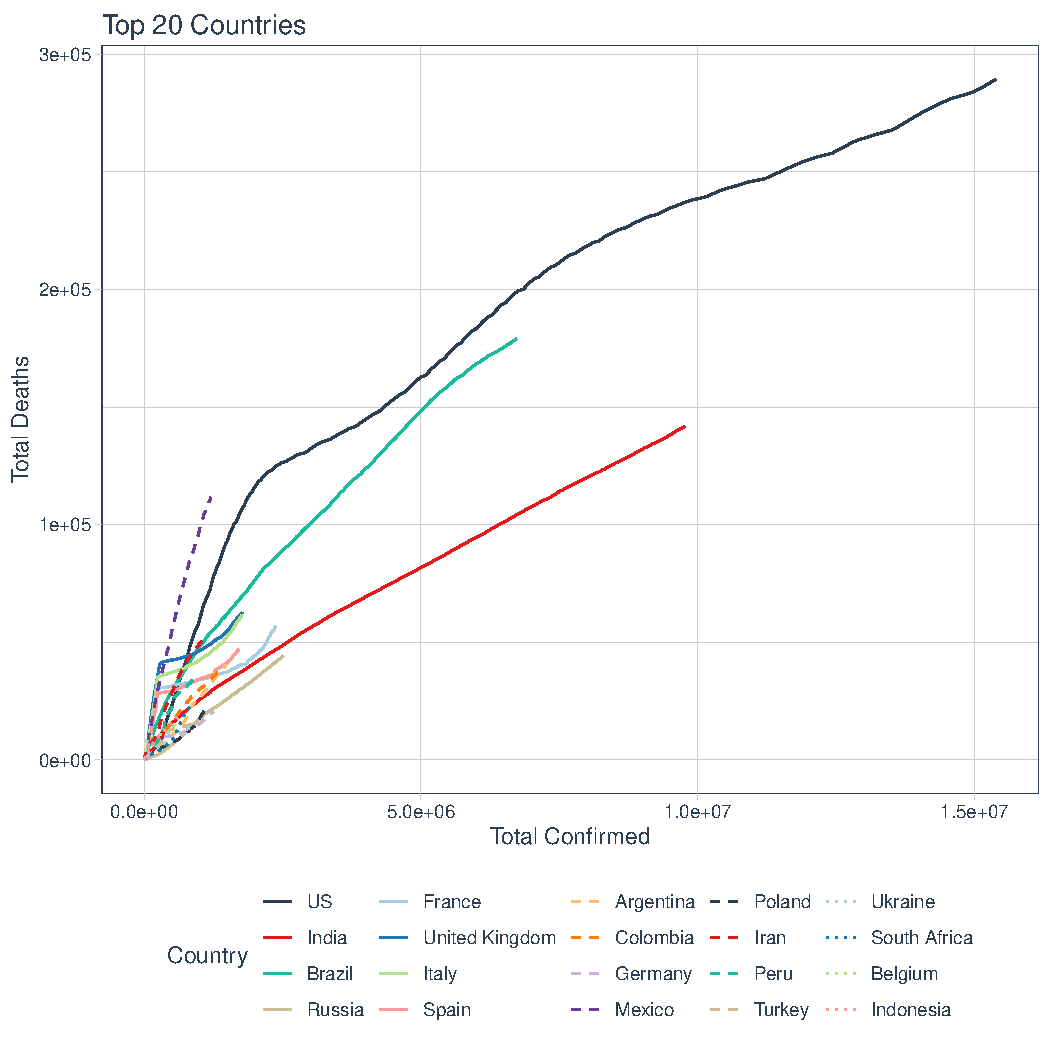
\includegraphics[width=\linewidth]{images/top_20_countries.pdf}
    \caption{Total Deaths vs Total Confirmed}
    \label{fig:top_20_countries}
\end{figure}
\newpage

As we see in Figure 4, only four countries out of twenty appear to have a different trend from the rest. Mexico is the first country that seems to have the most deaths compared to confirmed cases. In other words, Mexico has the steepest line of deaths vs confirmed cases. This could indicate that Mexico is a country with a very high death rate. After Mexico, the second steepest line is that of the US (black line).

The US tends to have a similar trend with Mexico but it is the country with the highest number of confirmed cases thus leading to a big number of deaths. Finally, the green line which depicts Brazil is quite similar to that of US, but it does not have such a big number of confirmed cases and deaths as the US due to a smaller population or stricter measures.

\newpage

\subsection{Based on Death Rates}

\begin{minted}[bgcolor=bg, fontsize=\scriptsize]{R}
#Sort the latest data by death rate, and if tie, by confirmed
countries_with_highest_death_rate <- data %>% filter(date==max(date)
  & Country != 'World' & confirmed >= 5000) %>%
  select(Country, confirmed, confirmed.ind, present.confirmed,
         deaths, deaths.inc, death.rate) %>%
  arrange(desc(death.rate, confirmed))
  countries_with_highest_rate %>% head(20)
  
#Infection-Fatality-Rate Evolution
ggplot(filter(data, Country %in% top.countries & confirmed >= 5000), 
              aes(x=date, y=death.rate)) +
  stat_summary(geom = "line",fun.y = mean, size= 1.2, colour='red') +
  xlab('Date') + ylab('Infection-Fatality-Rate (%)') + 
  labs(title='Infection-Fatality-Rate Evolution') +
  geom_line(aes(color=Country, linetype=Country)) +
  ylim(c(0, 18)) + 
  theme_tq() + 
  scale_color_tq()
\end{minted}

\begin{table}[!h]
\caption{\label{tab:}Top 20 Countries with Highest Infection Fatality rate - 2020-12-09}
\centering
\fontsize{7}{9}\selectfont
\begin{tabular}[t]{llrrrrrr}
\toprule
  & Country & confirmed & confirmed.ind & present.confirmed & deaths & deaths.inc & death.rate\\
\midrule
\cellcolor{gray!6}{1} & \cellcolor{gray!6}{Mexico} & \cellcolor{gray!6}{1,205,229} & \cellcolor{gray!6}{11,974} & \cellcolor{gray!6}{1,093,574} & \cellcolor{gray!6}{111,655} & \cellcolor{gray!6}{781} & \cellcolor{gray!6}{9.264\%}\\
2 & Ecuador & 199,228 & 476 & 185,414 & 13,814 & 20 & 6.934\%\\
\cellcolor{gray!6}{3} & \cellcolor{gray!6}{Sudan} & \cellcolor{gray!6}{20,084} & \cellcolor{gray!6}{337} & \cellcolor{gray!6}{18,777} & \cellcolor{gray!6}{1,307} & \cellcolor{gray!6}{6} & \cellcolor{gray!6}{6.508\%}\\
4 & Bolivia & 146,060 & 214 & 137,056 & 9,004 & 2 & 6.165\%\\
\cellcolor{gray!6}{5} & \cellcolor{gray!6}{Egypt} & \cellcolor{gray!6}{119,702} & \cellcolor{gray!6}{421} & \cellcolor{gray!6}{112,870} & \cellcolor{gray!6}{6,832} & \cellcolor{gray!6}{19} & \cellcolor{gray!6}{5.708\%}\\
\addlinespace
6 & Syria & 8,675 & 95 & 8,210 & 465 & 7 & 5.360\%\\
\cellcolor{gray!6}{7} & \cellcolor{gray!6}{China} & \cellcolor{gray!6}{93,898} & \cellcolor{gray!6}{116} & \cellcolor{gray!6}{89,150} & \cellcolor{gray!6}{4,748} & \cellcolor{gray!6}{2} & \cellcolor{gray!6}{5.057\%}\\
8 & Iran & 1,072,620 & 10,223 & 1,021,408 & 51,212 & 295 & 4.774\%\\
\cellcolor{gray!6}{9} & \cellcolor{gray!6}{Afghanistan} & \cellcolor{gray!6}{47,851} & \cellcolor{gray!6}{135} & \cellcolor{gray!6}{45,932} & \cellcolor{gray!6}{1,919} & \cellcolor{gray!6}{13} & \cellcolor{gray!6}{4.010\%}\\
10 & Peru & 976,621 & 2,709 & 940,220 & 36,401 & 127 & 3.727\%\\
\addlinespace
\cellcolor{gray!6}{11} & \cellcolor{gray!6}{United Kingdom} & \cellcolor{gray!6}{1,771,545} & \cellcolor{gray!6}{16,634} & \cellcolor{gray!6}{1,708,882} & \cellcolor{gray!6}{62,663} & \cellcolor{gray!6}{533} & \cellcolor{gray!6}{3.537\%}\\
12 & Italy & 1,770,149 & 12,755 & 1,708,410 & 61,739 & 499 & 3.488\%\\
\cellcolor{gray!6}{13} & \cellcolor{gray!6}{Tunisia} & \cellcolor{gray!6}{106,856} & \cellcolor{gray!6}{1,411} & \cellcolor{gray!6}{103,139} & \cellcolor{gray!6}{3,717} & \cellcolor{gray!6}{49} & \cellcolor{gray!6}{3.479\%}\\
14 & Guatemala & 127,127 & 654 & 122,816 & 4,311 & 25 & 3.391\%\\
\cellcolor{gray!6}{15} & \cellcolor{gray!6}{Mali} & \cellcolor{gray!6}{5,469} & \cellcolor{gray!6}{27} & \cellcolor{gray!6}{5,288} & \cellcolor{gray!6}{181} & \cellcolor{gray!6}{1} & \cellcolor{gray!6}{3.310\%}\\
\addlinespace
16 & Australia & 28,000 & 7 & 27,092 & 908 & 0 & 3.243\%\\
\cellcolor{gray!6}{17} & \cellcolor{gray!6}{Bosnia and Herzegovina} & \cellcolor{gray!6}{97,317} & \cellcolor{gray!6}{1,296} & \cellcolor{gray!6}{94,166} & \cellcolor{gray!6}{3,151} & \cellcolor{gray!6}{70} & \cellcolor{gray!6}{3.238\%}\\
18 & Bulgaria & 171,493 & 3,328 & 166,210 & 5,283 & 127 & 3.081\%\\
\cellcolor{gray!6}{19} & \cellcolor{gray!6}{Malawi} & \cellcolor{gray!6}{6,051} & \cellcolor{gray!6}{0} & \cellcolor{gray!6}{5,865} & \cellcolor{gray!6}{186} & \cellcolor{gray!6}{0} & \cellcolor{gray!6}{3.074\%}\\
20 & Indonesia & 592,900 & 6,058 & 574,729 & 18,171 & 171 & 3.065\%\\
\bottomrule
\end{tabular}
\end{table}
Table 5 shows the top 20 countries with the highest infection-fatality rate as of 2020-12-09 while Figure 5 shows the infection-fatality rate evolution. The infection-fatality rate is the ratio between the of the number of deaths and the number of confirmed cases. The average death rate for these countries is 4.521\% and the red line in Figure 5 depicts the average infection-fatality rate evolution of those 20 countries.

\begin{figure}[!h]
    \centering
    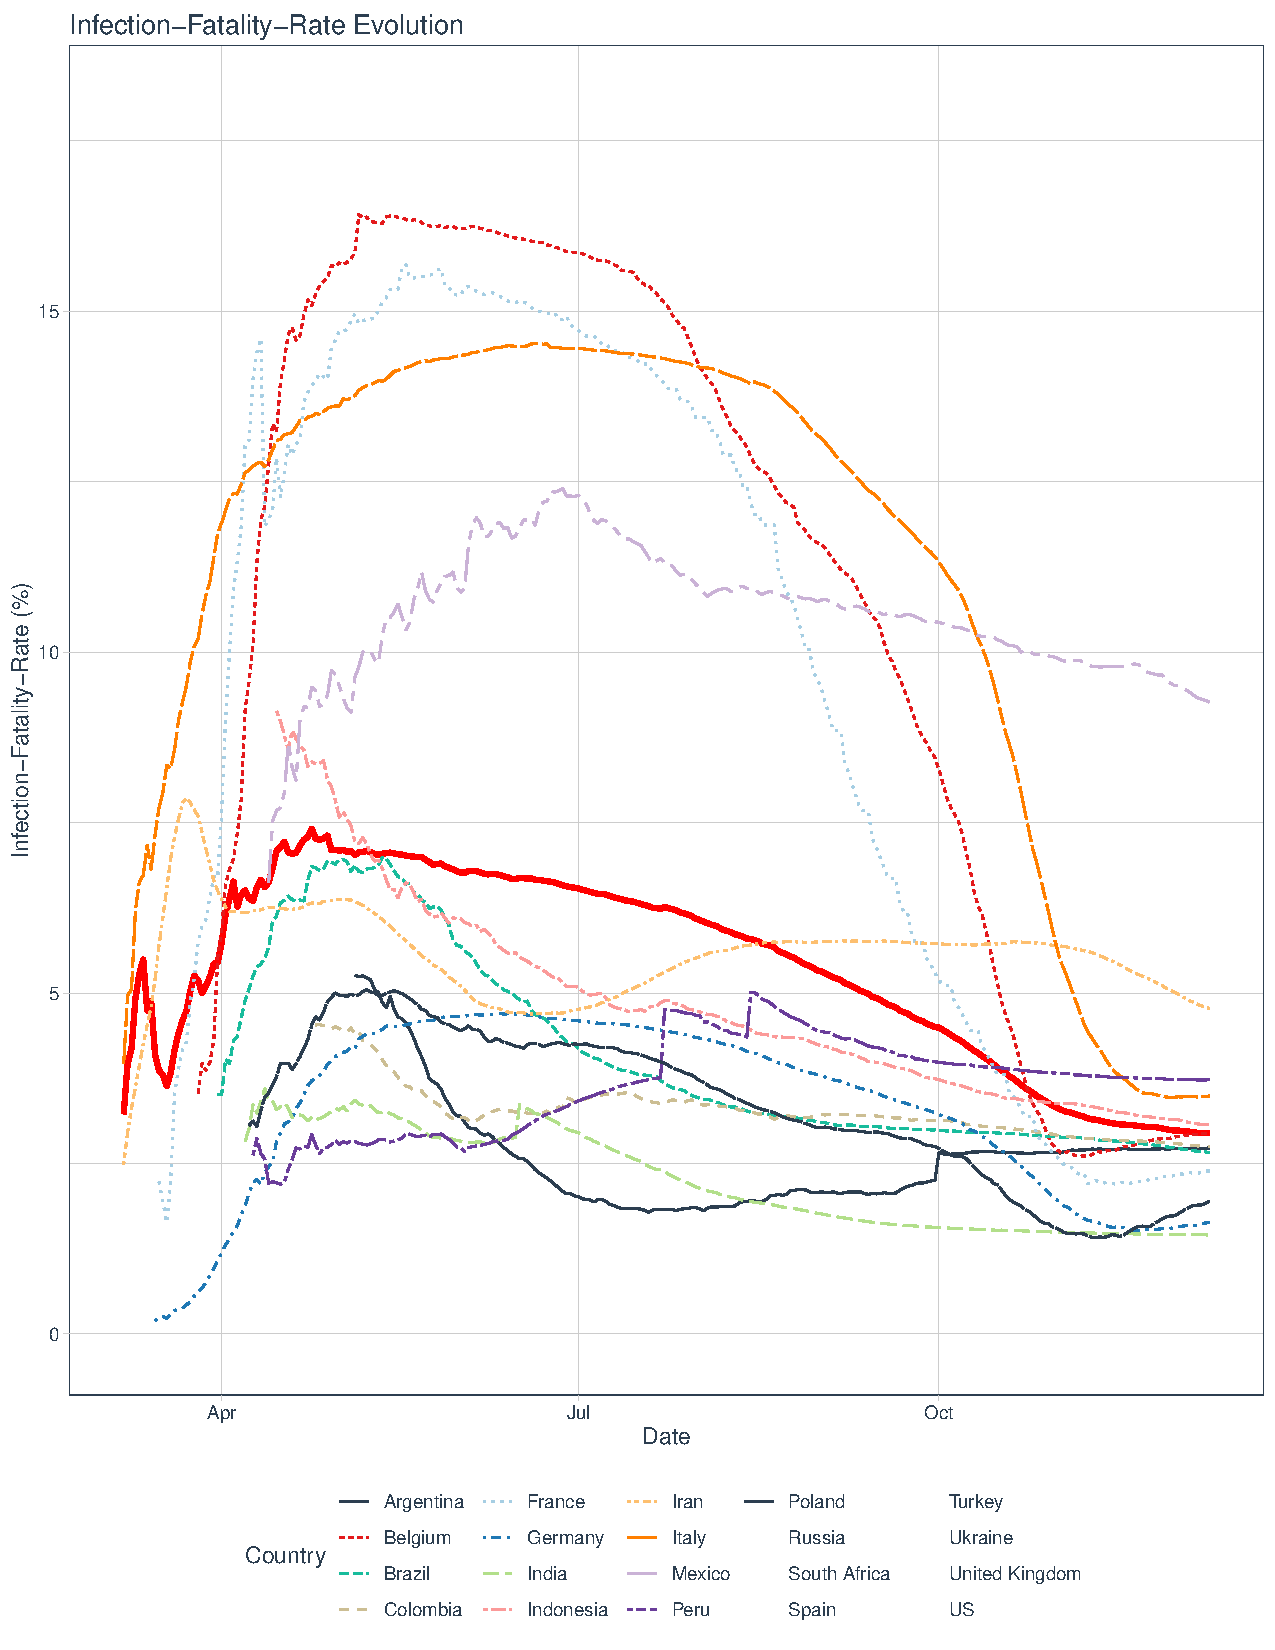
\includegraphics[width=\linewidth]{images/infection_fertility_evolution.pdf}
    \caption{Infection-Fatality-Rate Evolution of top 20 countries}
    \label{fig:top_20_countries}
\end{figure}

The country with the highest death rate is Mexico (9.264\%), whereas the country with the smallest rate is Indonesia (3.065\%). The death rate could be an indicator of the healthcare quality of each country. It is observed that most countries, with the highest death rates, are not developed ones perhaps proving that the high death rates could be attributed to lack of healthcare and perhaps poverty.

%\input{results2.tex}
%\input{conclusion.tex}



%\newpage
%\bibliographystyle{IEEEtran}
%\bibliography{refs}
\end{document}